\documentclass{article}
\usepackage[utf8]{inputenc}
\usepackage[portuges]{babel}
\usepackage[a4paper, total={7in, 9in}]{geometry}
\usepackage{graphicx}
\usepackage{float}
\usepackage{fancyvrb}
\usepackage{indentfirst}
\usepackage{amsmath}
\usepackage{hyperref}

\usepackage[dvipsnames,table,xcdraw]{xcolor}
\usepackage{color}
\usepackage{minted}
\usemintedstyle{friendly}
\definecolor{bg}{rgb}{0.96,0.96,0.96}

\newcommand{\question}[1]{
    {\large \textbf{Q: #1}}
    \\
}

\newcommand{\titleRule}{
    \rule{\linewidth}{0.5mm} \\ [0.25cm]
}

\begin{document}

\begin{titlepage}
    \center
    \begin{figure}[H]
        \centering
        
\includegraphics[width=4cm]{UM_EENG.jpg}
    \end{figure}
    \textsc{\LARGE Universidade do Minho} \\ [1.5cm]
    \textsc{\Large Mestrado Integrado em Engenharia Informática} \\ [0.5cm]
    \textsc{\large Scripting no Processamento de Linguagem Natural} \\ [0.5cm]

    \titleRule
    {\huge \bfseries RSS Spider}
    \titleRule

    João Pedro Ferreira Vieira A78468 \\
    Miguel Miranda Quaresma A77049 \\[0.25cm]

    \today
\end{titlepage}

\tableofcontents

\newpage

\section{Introdução}

A quantidade de informação existente atualmente torna cada vez mais importante a existência de mecanismos que permitam processar
esta informação e, subsequentemente, procurar por documentos com base em termos. Esta pesquisa deve no entanto, ter em conta a
importância dos termos utilizados no texto, favorecendo nomes a determinantes, sendo útil o uso de algoritmos como \emph{TF-IDF} que 
têm em conta a frequência de um dado termo no conjunto de documentos. 
A presente ferramenta recorre a estes mecanismos para indexar um conjunto de documentos e permitir ao utilizador realizar pesquisas
nos mesmos.

\section{Algortimo de pesquisa : \emph{TF-IDF}}

O algoritmo utilizado neste trabalho é o \emph{TF-IDF} (\emph{Term Frequency - Inverse Document Frequency}) consiste numa estatística numérica com o propósito de refletir a importância que uma palavra tem num documento de uma determinada coleção. Este tipo de algoritmo é bastante usado por motores de busca como uma ferramenta que classifica e ordena documentos tendo em conta uma \emph{query} pesquisada pelo utilizador.

Para explicar o processo do algoritmo podemos dividir o mesmo em duas partes, \emph{TF} e \emph{IDF}:

\subsection{\emph{TF (Term Frequency)}}

Supondo que temos um conjunto de documentos (textos) e pretendemos ordenar os documentos por relevância tendo em conta uma pesquisa (uma palavra ou um conjunto de palavras), uma solução pode passar por contar o número de vezes que cada termo ocorre em cada documento. O número de vezes que um termo aparece num dado documento é denominado de \textbf{\emph{term frequency}}.

Tendo em conta que cada documento tem um tamanho diferente (\emph{length}), isso torna possível e expectável que um dado termo apareça mais vezes num texto maior do que num com menos palavras. Sendo assim, a frequência de um termo é normalmente dividida pelo tamanho do documento:

\[
    TF(termo) = \frac{\text{Número de vezes que o termo aparece no documento}}{\text{Número total de termos no documento}}
\]

\subsection{\emph{IDF (Inverse Document Frequency)}}

Esta métrica pretende medir a importância de um termo. Tendo em conta apenas o cálculo de \emph{TF}, todos os termos são considerados igualmente importantes, no entanto, é fácil de perceber que certos termos como "o", "a", "de" ou "no" podem aparecer num documento muitas vezes mas a sua importância acaba por ser pouca. Desta forma, necessitamos de atribuir menor relevância a termos muito frequentes e atribuir maior importância a termos raros, o que é conseguido através da fórmula:

\[
    IDF(termo) = \log_{e} (\frac{\text{Número total de documentos}}{\text{Número de documentos que contêm o termo}})
\]

\section{RSS Spider}
A aplicação desenvolvida apresenta dois modos de funcionamento, o primeiro que consiste em requisitar um conjunto de documentos referenciados num \texttt{RSS Feed}
e criar uma base de dados constituída por estes documentos, após serem processados e indexados. O segundo modo de funcionamento recorre ao índice criado 
anteriormente para efetuar uma pesquisa nos documentos armazenados tendo por base uma \textit{query} introduzida pelo utilizador. 
O \emph{RSS Feed} utilizado para este projeto foi \url{https://blog.filippo.io/rss/}, sendo que o mesmo programa poderá facilmente ser extendido a qualquer \emph{feed} desde que adaptado à estrutura do mesmo.

\subsection{RSS Feed}
\label{rss_format}
O formato \textit{RSS}, \textbf{R}eally \textbf{S}imple \textbf{S}yndication, define uma forma de apresentar conteúdo que seja relevante, sendo de especial relevância
em \textit{sites} que estejam constantemente a produzir novos artigos/documentos. 
O formato é escrito em XML sendo relevante destacar alguns elementos de maior importância para facilitar a compreensão da ferramenta desenvolvida.
É importante realçar que, dado não haver um \texttt{standard} aceite como universal para o \texttt{RSS Feed}, existem variações no formato utilizado, como tal
a descrição aqui apresentada deve ser considerada apenas para propósitos académicos:
\begin{itemize}
    \item \texttt{channel}: contém a descrição do \textit{feed}
    \begin{itemize}
        \item \texttt{item}: representa um artigo/documento individual
        \begin{itemize}
            \item \texttt{link}: hiperligação para o artigo/documento
            \item \texttt{description}: descrição do item
            \item \texttt{content}: conteúdo do artigo/documento
            \item \texttt{category}: categoria do documento
        \end{itemize}
    \end{itemize}
\end{itemize}


\subsection{Atualização da base de dados}
A atualização da base de dados de documentos consiste em obter os documentos referenciados no RSS \textit{Feed} e processá-los calculando a porção \textbf{TF} (\textit{Term Frequency}) dos termos presentes em cada documento, armazenando ambos.

Para obter os documentos, é invocada a função \texttt{refreshDB()} que efetua, com recurso à biblioteca \textit{Requests}, um pedido \texttt{HTTP GET} ao URL que contém 
o \textit{feed}.

\begin{minted}[bgcolor=bg, 
               framesep=2mm,
               %linenos,
               breaklines,
               breakautoindent=true,
               breaksymbolleft=\raisebox{0.8ex}{\tiny\hookrightarrow},
               breaksymbolindentleft=0pt,
               breaksymbolsepleft=1pt,
               breaksymbolright=\raisebox{0.8ex}{\tiny\hookleftarrow},
               breaksymbolindentright=0pt,
               breaksymbolsepright=1pt
]{text}
updated_feed = requests.get(rss_url).content 
\end{minted}

O conteúdo obtido é processado com recurso à biblioteca \textit{BeautifulSoup}, que permite efetuar o \textit{parsing} de HTML, XML (e outros formatos). 
Neste caso, o formato é XML, sendo esse o modo escolhido para o \textit{parsing}.
Dado o formato anteriormente descrito (conf. \ref{rss_format}), é efetuada uma procura por todos os elementos do tipo \textit{item} e, para cada um, é
identificado o \textit{link} do \textit{post}, que é depois requisitado, mais uma vez, com recurso à biblioteca \textit{Requests}:

\begin{minted}[bgcolor=bg, 
               framesep=2mm,
               %linenos,
               breaklines,
               breakautoindent=true,
               breaksymbolleft=\raisebox{0.8ex}{\tiny\hookrightarrow},
               breaksymbolindentleft=0pt,
               breaksymbolsepleft=1pt,
               breaksymbolright=\raisebox{0.8ex}{\tiny\hookleftarrow},
               breaksymbolindentright=0pt,
               breaksymbolsepright=1pt
]{text}
parse_tree = BeautifulSoup(updated_feed, "xml")
news = parse_tree.find_all("item")
links = [new.find("link").text for new in news]
\end{minted}

Cada documento é processado pela função \texttt{procDoc(link)} que, após requisitar o recurso indicado no URL passado como argumento (\texttt{link}), realiza o
\textit{parse} do mesmo, obtendo as \textit{tags} mais relevantes: \texttt{p, pre, h1, h2, h3, h4, ul, ol, blockquote} e ignorando o conteúdo presente no \textit{header} e \textit{footer},
caraterísticos do formato HTML:
\begin{minted}[bgcolor=bg, 
               framesep=2mm,
               %linenos,
               breaklines,
               breakautoindent=true,
               breaksymbolleft=\raisebox{0.8ex}{\tiny\hookrightarrow},
               breaksymbolindentleft=0pt,
               breaksymbolsepleft=1pt,
               breaksymbolright=\raisebox{0.8ex}{\tiny\hookleftarrow},
               breaksymbolindentright=0pt,
               breaksymbolsepright=1pt
]{text}
textsection = soup.find('section','post-content')
find = textsection.find_all(["p", "pre", "h2", "h3", "h4", "ul", "ol", "blockquote"],
    recursive=False) 
\end{minted}
Por forma a facilitar a visualização posterior dos documentos armazenados, as secções obtidas são mantidas em formato HTML, tendo sido gerado um ficheiro
CSS que permite formatar os documentos para facilitar a sua leitura/consulta: 
\begin{figure}[H]
    \centering
    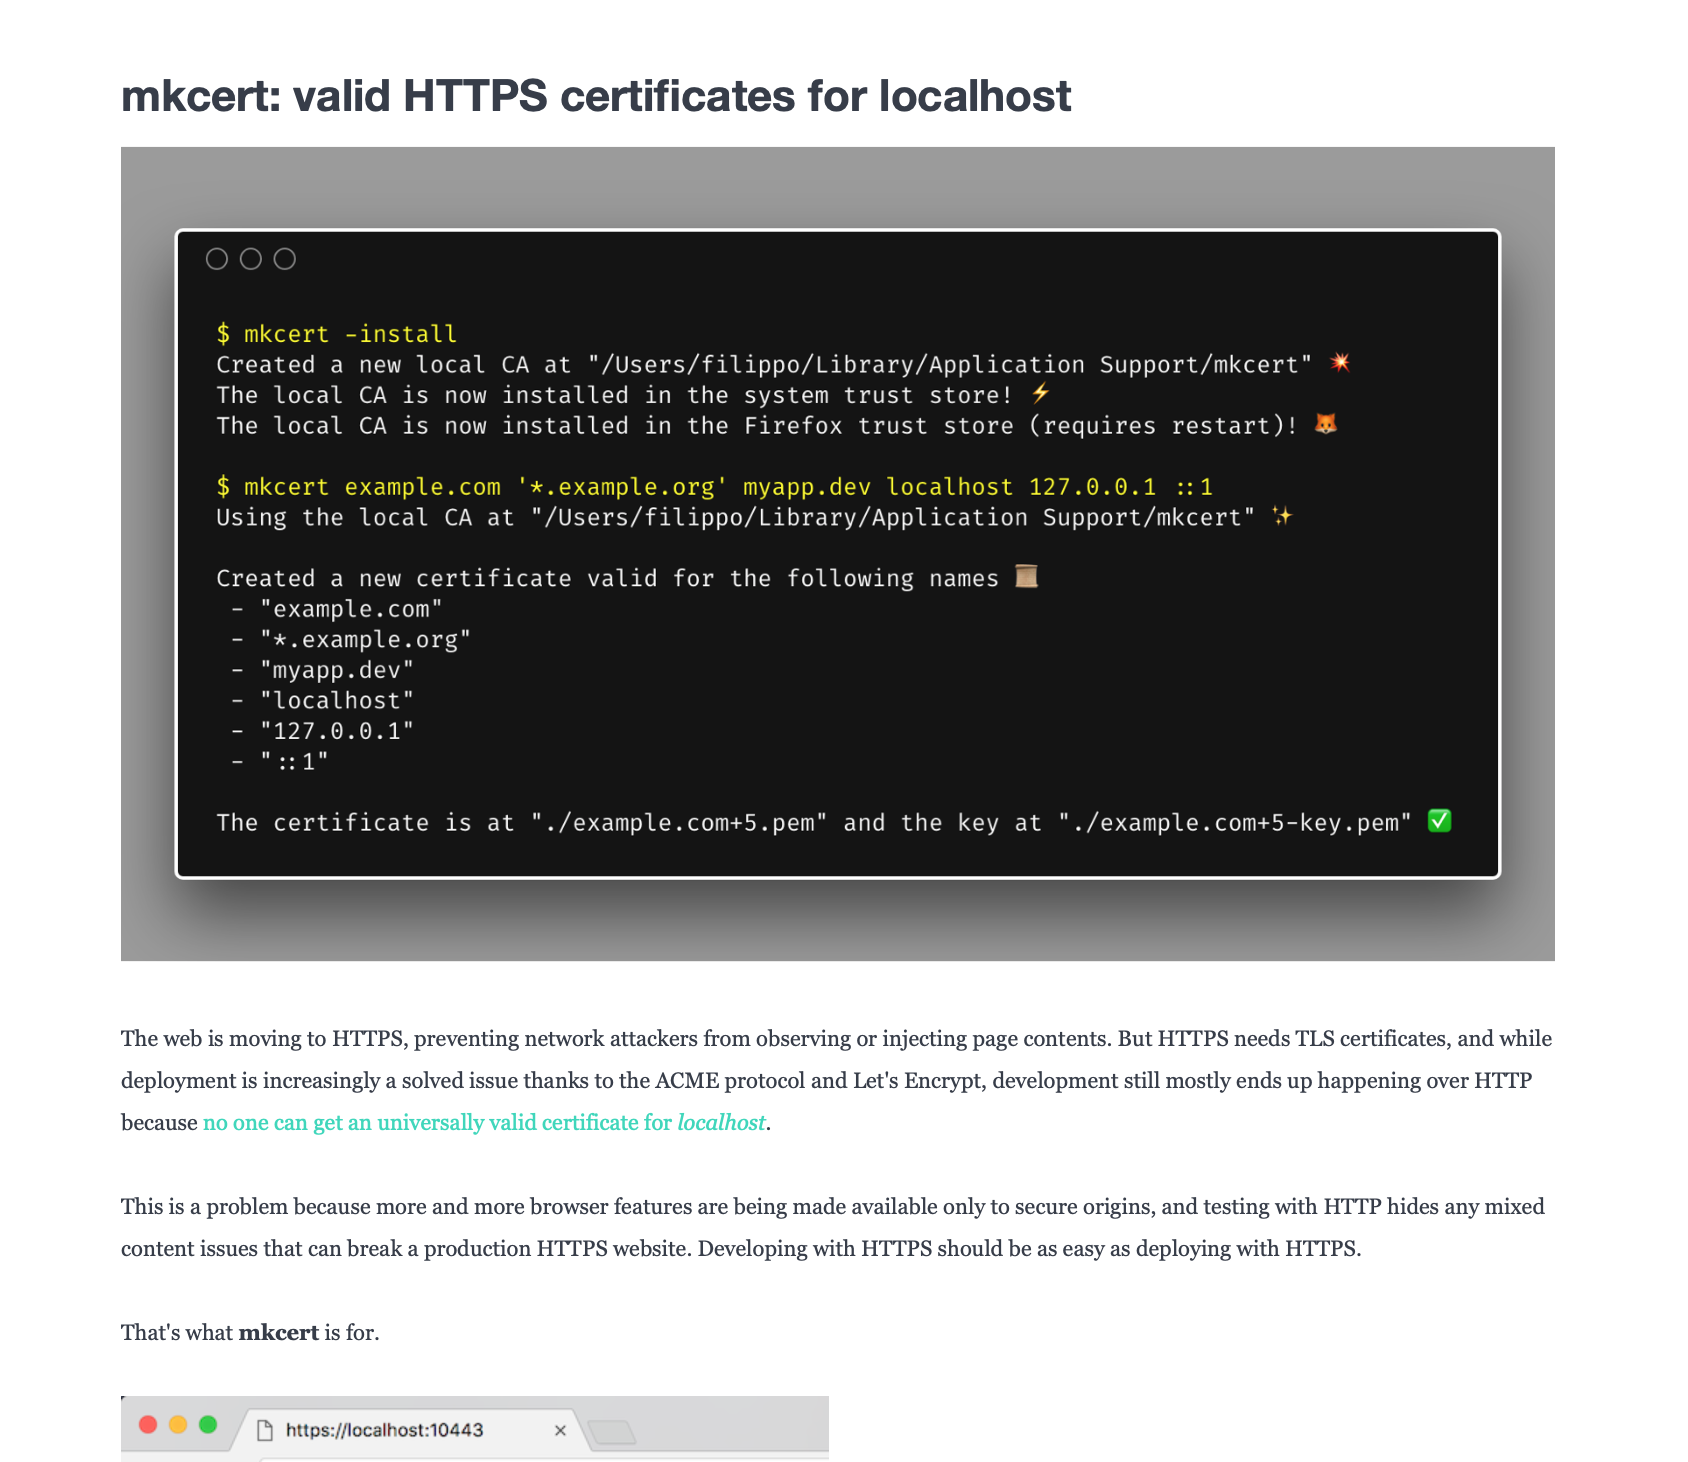
\includegraphics[width=12cm]{mkcert_example.png}
    \caption{Documento formatado para leitura}
\end{figure}

Para além do armazenamento dos ficheiros é ainda criado um indíce (\texttt{doc\_index}) que associa os termos, e respetivas frequências, a cada documento, que é usado quando um utilizador deseja efetuar uma pesquisa.

\begin{figure}[H]
    \centering
    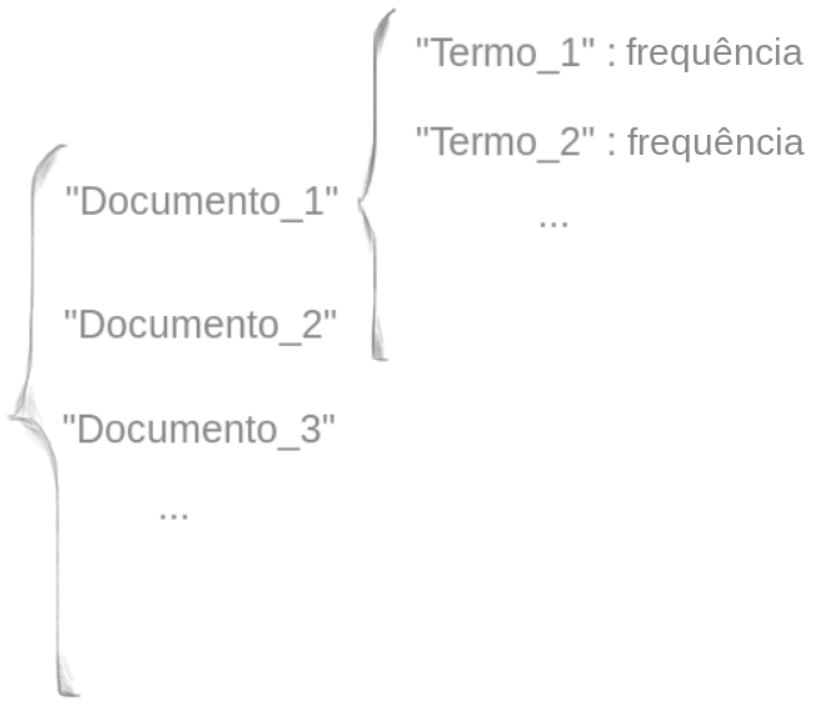
\includegraphics[width=7cm]{formato_dicionario.png}
    \caption{Formato do dicionário/índice}
\end{figure}

Para documento, é invocada a função \texttt{buildDocIndex(filename, text)}, que recebe o nome do documento bem como o seu conteúdo, isento das \textit{tags} HTML e
divide este texto nos seus termos(palavras) constituintes, calculando para um a frequência no presente documento. Por forma a evitar a diferenciação entre termos
que estejam em letra maiúscula ou minúscula, ou que sejam procedidos de pontuação, o texto é previamente convertido para \textit{lower case} sendo também removida
a pontuação nele existente:

\begin{minted}[bgcolor=bg, 
               framesep=2mm,
               %linenos,
               breaklines,
               breakautoindent=true,
               breaksymbolleft=\raisebox{0.8ex}{\tiny\hookrightarrow},
               breaksymbolindentleft=0pt,
               breaksymbolsepleft=1pt,
               breaksymbolright=\raisebox{0.8ex}{\tiny\hookleftarrow},
               breaksymbolindentright=0pt,
               breaksymbolsepright=1pt
]{text}
text = re.sub(r'\p{punct}', r'', text)
text = text.lower()
terms = re.split(r'\s+', text) 
\end{minted}

Após serem processados todos os documentos o índice é armazenado, com recurso ao módulo \textit{Pickle}, no ficheiro \texttt{rsspider.index}:

\begin{minted}[bgcolor=bg, 
               framesep=2mm,
               %linenos,
               breaklines,
               breakautoindent=true,
               breaksymbolleft=\raisebox{0.8ex}{\tiny\hookrightarrow},
               breaksymbolindentleft=0pt,
               breaksymbolsepleft=1pt,
               breaksymbolright=\raisebox{0.8ex}{\tiny\hookleftarrow},
               breaksymbolindentright=0pt,
               breaksymbolsepright=1pt
]{text}
index_dump = "rsspider.index"
...
index_db = open(index_dump, "wb")
pickle.dump(doc_index, index_db) 
\end{minted}


\subsection{Procura e consulta de documentos}

Para processar uma dada \emph{query} de pesquisa do utilizador à aplicação é utilizada a função \texttt{procRequest()} que recebe como parâmetro os termos de pesquisa inseridos.

Inicialmente, começa-se por carregar para memória o índice criado e explicado na secção anterior, novamente com o auxílio do módulo \emph{Pickle}.

\begin{minted}[bgcolor=bg, 
               framesep=2mm,
               %linenos,
               breaklines,
               breakautoindent=true,
               breaksymbolleft=\raisebox{0.8ex}{\tiny\hookrightarrow},
               breaksymbolindentleft=0pt,
               breaksymbolsepleft=1pt,
               breaksymbolright=\raisebox{0.8ex}{\tiny\hookleftarrow},
               breaksymbolindentright=0pt,
               breaksymbolsepright=1pt
]{text}
indexer = open(index_dump, "rb")
doc_index = pickle.load(indexer)
\end{minted}

O processo para obter e ordenar os documentos relacionados começa por filtrar os documentos que possuem qualquer um dos termos pesquisados, obtendo para cada um
a frequência dos termos encontrados. Adicionalmente, para cada um destes termos é calculado o \textbf{IDF} correspondente e, sendo este valor combinado com a 
sua frequência em cada documento. A cada documento será então associado um valor que é tanto maior quanto mais relevante este documento for tendo em conta os termos
de pesquisa introduzidos pelo utilizador, sendo este o valor utilizado na ordenação dos documentos que são apresentados ao utilizador. Os somatório dos diferentes 
\textbf{TF-IDF}'s dos termos comuns ao documento e \textit{query} corresponderão, por isso, a este valor que é atualizado da seguinte maneira: 
"\textit{valor\_anterior + IDF * frequência\_do\_termo\_no\_documento}", sendo que o \emph{valor\_anterior} toma o valor de 0 na primeira vez que a fórmula é 
utilizada. 

\begin{minted}[bgcolor=bg, 
               framesep=2mm,
               %linenos,
               breaklines,
               breakautoindent=true,
               breaksymbolleft=\raisebox{0.8ex}{\tiny\hookrightarrow},
               breaksymbolindentleft=0pt,
               breaksymbolsepleft=1pt,
               breaksymbolright=\raisebox{0.8ex}{\tiny\hookleftarrow},
               breaksymbolindentright=0pt,
               breaksymbolsepright=1pt
]{text}
doc_scale = {}
for term in search_terms:
    doc_term = {}
    for doc in doc_index:
        if term in doc_index[doc]:
            doc_term[doc] = doc_index[doc][term]
    try:
        idf = math.log(tot_docs/len(doc_term))
    except ZeroDivisionError:
        idf = 0
    for doc in doc_term:
        doc_scale[doc] = doc_scale.get(doc, 0) + idf*doc_term[doc]
relevant_docs = sorted(doc_scale.keys(), key=doc_scale.get, reverse=True)
\end{minted}

\section{Interface com o utilizador}

Para tornar mais simpática e melhorar a experiência do utilizador da aplicação, decidimos criar uma interface gráfica para a aplicação desenvolvida. Para tal, utilizamos a biblioteca \emph{TkInter}, que é a biblioteca GUI (\emph{Guide User Interface}) \emph{standard} para o \emph{Python}. Através da utilização simultânea de \emph{Python} combinada com o \emph{TkInter} conseguimos uma forma rápida e fácil de fazer interfaces para aplicações.

Um exemplo da utilização da interface é apresentado de seguida.

\begin{figure}[H]
    \centering
    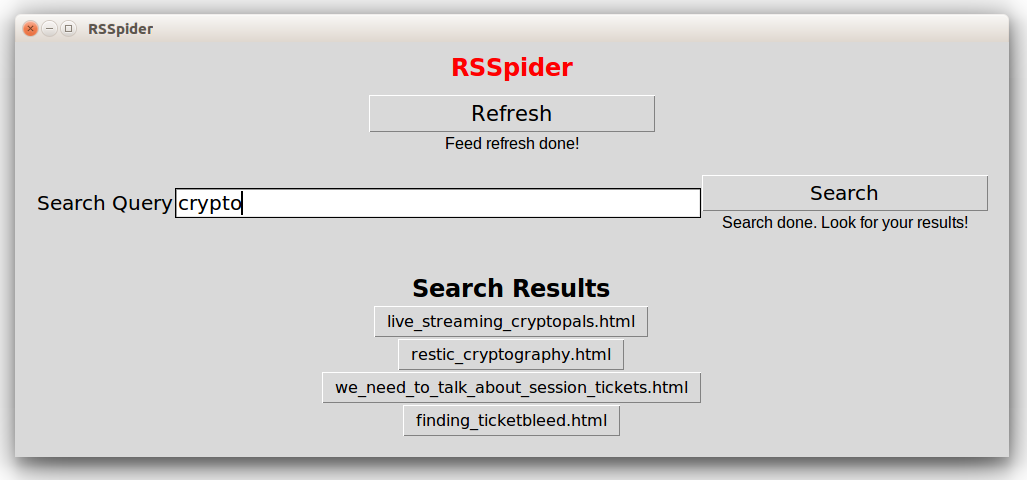
\includegraphics[width=14cm]{interface.png}
    \caption{Formato do dicionário/índice}
\end{figure}

\begin{itemize}
    \item O botão \textbf{Refresh} faz a atualização (ou construção caso seja a primeira vez) da base de dados de documentos e constrói o dicionário explicado anteriormente e guardado em \texttt{rsspider.index}.
    \item O botão \textbf{Search} faz a procura e ordenação dos documentos relacionados com uma dada \emph{query} inserida pelo utilizador. Para efetuar isto é obtida inicialmente a \emph{query} do campo em causa, processando-a depois de forma a remover todas as pontuações presentes na mesma, e obtendo a lista de termos, através da separação por espaços e filtragem dos elementos com um tamanho superior a 0. Caso a lista obtida tenha um tamanho nulo, é indicado que a procura é inválida.
    \begin{minted}[bgcolor=bg, 
               framesep=2mm,
               %linenos,
               breaklines,
               breakautoindent=true,
               breaksymbolleft=\raisebox{0.8ex}{\tiny\hookrightarrow},
               breaksymbolindentleft=0pt,
               breaksymbolsepleft=1pt,
               breaksymbolright=\raisebox{0.8ex}{\tiny\hookleftarrow},
               breaksymbolindentright=0pt,
               breaksymbolsepright=1pt
]{text}
query = self.query_string.get()
query = re.sub(r'\p{punct}', r'', query)
query = list(filter(lambda x: len(x)>0, re.split(r'\s+', query)))
\end{minted}
    \item Para cada documento pertencente ao resultado obtido, é criado um botão para o mesmo. Através da utilização do módulo \emph{webbrowser (Convenient Web-browser controller)}, ao clicar num desses botões é aberto o documento HTML guardado na base de dados no \emph{browser} definido pelo utilizador para abrir documentos desse tipo.
    \begin{minted}[bgcolor=bg, 
               framesep=2mm,
               %linenos,
               breaklines,
               breakautoindent=true,
               breaksymbolleft=\raisebox{0.8ex}{\tiny\hookrightarrow},
               breaksymbolindentleft=0pt,
               breaksymbolsepleft=1pt,
               breaksymbolright=\raisebox{0.8ex}{\tiny\hookleftarrow},
               breaksymbolindentright=0pt,
               breaksymbolsepright=1pt
]{text}
def openDocument(self, filename):
    webbrowser.open('file://' + os.path.realpath(filename))
\end{minted}
    
\end{itemize}

\section{Conclusão}
A ferramenta implementada permite efetuar uma pesquisa eficiente de um RSS \textit{feed}, automatizando a obtenção de documentos e armazenando os mesmos para que 
possam ser consultados \textit{offline} num formato legível. Adicionalmente, e tendo \textit{performance} em mente, a operação de indexação é efetuada na atualização 
da base de dados de documentos, permitindo que as pesquisas sejam realizadas em tempo aceitável sem detrimento para a experiência do utilizador.
Por outro lado, a ferramenta desenvolvida apresenta uma escalabilidade que permite que seja facilmente adaptada a outro \textit{feed} que o utilizador deseje, sendo
esta uma funcionalidade que deve ser considerada numa versão futura da ferramenta. 
\end{document}